\def\pointsize{2pt}

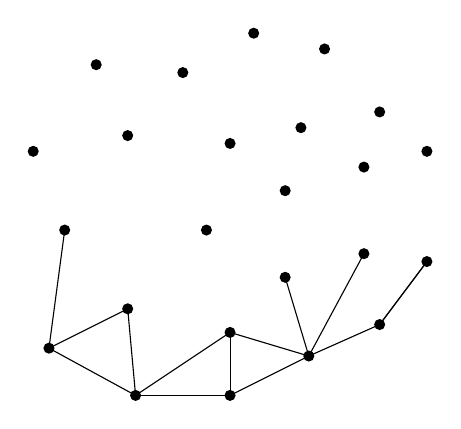
\begin{tikzpicture}[
  scale=1]

\coordinate (p1) at (1,1);
\coordinate (p2) at (2.1,0.4);
\coordinate (p3) at (3.3,0.4);
\coordinate (p4) at (4.3,0.9);
\coordinate (p5) at (5.2,1.3);
\coordinate (p6) at (5.8,2.1);
\coordinate (p7) at (5.8,3.5);
\coordinate (p8) at (5.2,4);
\coordinate (p9) at (4.5,4.8);
\coordinate (p10) at (3.6,5);
\coordinate (p11) at (2.7,4.5);
\coordinate (p12) at (1.6,4.6);
\coordinate (p13) at (0.8,3.5);
\coordinate (p14) at (1.2,2.5);
\coordinate (p15) at (2,1.5);
\coordinate (p16) at (3.3,1.2);
\coordinate (p17) at (4,1.9);
\coordinate (p18) at (5,2.2);
\coordinate (p19) at (5,3.3);
\coordinate (p20) at (4.2,3.8);
\coordinate (p21) at (3.3,3.6);
\coordinate (p22) at (2,3.7);
\coordinate (i) at (3,2.5);
\coordinate (j) at (4,3);

\fill (p1) circle (\pointsize);
\fill (p2) circle (\pointsize);
\fill (p3) circle (\pointsize);
\fill (p4) circle (\pointsize);
\fill (p5) circle (\pointsize);
\fill (p6) circle (\pointsize);
\fill (p7) circle (\pointsize);
\fill (p8) circle (\pointsize);
\fill (p9) circle (\pointsize);
\fill (p10) circle (\pointsize);
\fill (p11) circle (\pointsize);
\fill (p12) circle (\pointsize);
\fill (p13) circle (\pointsize);
\fill (p14) circle (\pointsize);
\fill (p15) circle (\pointsize);
\fill (p16) circle (\pointsize);
\fill (p17) circle (\pointsize);
\fill (p18) circle (\pointsize);
\fill (p19) circle (\pointsize);
\fill (p20) circle (\pointsize);
\fill (p21) circle (\pointsize);
\fill (p22) circle (\pointsize);
\fill (i) circle (\pointsize);
\fill (j) circle (\pointsize);

\draw (p1) -- (p2);
\draw (p1) -- (p14);
\draw (p1) -- (p15);
\draw (p2) -- (p3);
\draw (p2) -- (p15);
\draw (p2) -- (p16);
\draw (p3) -- (p4);
\draw (p3) -- (p16);
\draw (p4) -- (p5);
\draw (p4) -- (p16);
\draw (p4) -- (p17);
\draw (p4) -- (p18);
\draw (p5) -- (p6);
\draw (p5) -- (p6);


\end{tikzpicture}
%
%
%
%
%
%\def\dx{2}
%\def\xone{0}
%\def\xtwo{\xone+\dx}
%\def\xthree{\xtwo+\dx}
%\def\fluxone{2}
%\def\fluxtwo{1}
%\def\fluxthree{1}
%\def\yHone{-1}
%\def\yHtwo{0.5}
%\def\yHthree{0.5}
%\def\yLone{\yHone+\fluxone}
%\def\yLtwo{\yHtwo-\fluxtwo}
%\def\yLthree{\yHthree-\fluxthree}
%\def\ytitle{3}
%\def\yint{-3}
%\def\pointsize{2pt}
%\def\arrowlinewidth{1.5pt}
%\def\textdistancey{0.25}
%\def\textsep{0.5}
%\def\graphdistance{3.5*\dx}
%
%\begin{tikzpicture}[
%  scale=1,
%  myarrow/.style={
%    -latex,
%    line width=\arrowlinewidth}]
%
%% Left
%\coordinate[label=below:$\frac{m_1}{\dt}U_1^H$] (uH1) at (\xone,\yHone);
%\coordinate[label=above:$\frac{m_2}{\dt}U_2^H$] (uH2) at (\xtwo,\yHtwo);
%\coordinate[label=above:$\frac{m_3}{\dt}U_3^H$] (uH3) at (\xthree,\yHthree);
%\coordinate[label=above:$\frac{m_1}{\dt}U_1^L$] (uL1) at (\xone,\yLone);
%\coordinate[label=below:$\frac{m_2}{\dt}U_2^L$] (uL2) at (\xtwo,\yLtwo);
%\coordinate[label=below:$\frac{m_3}{\dt}U_3^L$] (uL3) at (\xthree,\yLthree);
%\coordinate[label=right:$\correctionfluxletter_1$] (p1) at ($0.5*(uH1)+0.5*(uL1)$);
%\coordinate[label=right:$\correctionfluxletter_2$] (p2) at ($0.5*(uH2)+0.5*(uL2)$);
%\coordinate[label=right:$\correctionfluxletter_3$] (p3) at ($0.5*(uH3)+0.5*(uL3)$);
%\fill (uH1) circle (\pointsize);
%\fill (uH2) circle (\pointsize);
%\fill (uH3) circle (\pointsize);
%\fill (uL1) circle (\pointsize);
%\fill (uL2) circle (\pointsize);
%\fill (uL3) circle (\pointsize);
%\draw[myarrow] (uL1) -- (uH1);
%\draw[myarrow] (uL2) -- (uH2);
%\draw[myarrow] (uL3) -- (uH3);
%\node at (\xtwo,\ytitle) {Antidiffusive Flux Definition:};
%\node at (\xtwo,\ytitle-\textsep) {$\frac{m_i}{\dt}U^H_i = \frac{m_i}{\dt}U^L_i
%  + \correctionfluxletter_i$};
%
%% Right
%\coordinate[label=below:$\frac{m_1}{\dt}U_1^H$] (uH1r) at (\graphdistance+\xone,\yHone);
%\coordinate[label=left:$\frac{m_2}{\dt}U_2^H$] (uH2r) at (\graphdistance+\xtwo,\yHtwo);
%\coordinate[label=above:$\frac{m_3}{\dt}U_3^H$] (uH3r) at (\graphdistance+\xthree,\yHthree);
%\coordinate[label=above:$\frac{m_1}{\dt}U_1^L$] (uL1r) at (\graphdistance+\xone,\yLone);
%\coordinate[label=below:$\frac{m_2}{\dt}U_2^L$] (uL2r) at (\graphdistance+\xtwo,\yLtwo);
%\coordinate[label=below:$\frac{m_3}{\dt}U_3^L$] (uL3r) at (\graphdistance+\xthree,\yLthree);
%\coordinate (uL2rplusp1) at (\graphdistance+\xtwo,\yLtwo+\fluxone);
%\coordinate[label=right:$\textcolor{red}{\correctionfluxentry_{1,2}}$] (p12) at ($0.5*(uH1r)+0.5*(uL1r)$);
%\coordinate[label=right:$\textcolor{red}{\correctionfluxentry_{2,1}}$] (p21) at ($0.5*(uL2r)+0.5*(uH2r)$);
%\coordinate[label=right:$\textcolor{blue}{\correctionfluxentry_{2,3}}$] (p23) at ($0.5*(uL2rplusp1)+0.5*(uH2r)$);
%\coordinate[label=right:$\textcolor{blue}{\correctionfluxentry_{3,2}}$] (p32) at ($0.5*(uL3r)+0.5*(uH3r)$);
%
%\fill (uH1r) circle (\pointsize);
%\fill (uH2r) circle (\pointsize);
%\fill (uH3r) circle (\pointsize);
%\fill (uL1r) circle (\pointsize);
%\fill (uL2r) circle (\pointsize);
%\fill (uL3r) circle (\pointsize);
%\draw[myarrow,red] (uL1r) -- (uH1r);
%\draw[myarrow,red] (uL2r) -- (uL2rplusp1);
%\draw[myarrow,blue] (uL2rplusp1) -- (uH2r);
%\draw[myarrow,blue] (uL3r) -- (uH3r);
%\node at (\graphdistance+\xtwo,\ytitle) {Antidiffusive Flux Decomposition:};
%\node at (\graphdistance+\xtwo,\ytitle-\textsep) {$\correctionfluxletter_i =
%  \sum\limits_j \correctionfluxentry\ij
%  \eqc \quad \correctionfluxentry\ji = -\correctionfluxentry\ij$};
%
%% Internodal plot
%\coordinate[label=below:$1$] (int1) at (\graphdistance+\xone,\yint);
%\coordinate[label=below:$2$] (int2) at (\graphdistance+\xtwo,\yint);
%\coordinate[label=below:$3$] (int3) at (\graphdistance+\xthree,\yint);
%
%\fill (int1) circle (\pointsize);
%\fill (int2) circle (\pointsize);
%\fill (int3) circle (\pointsize);
%
%\draw (int1) -- (int3);
%\draw[myarrow,color=red] (int1) arc (180:0:0.5*\dx);
%\draw[myarrow,color=blue] (int2) arc (180:0:0.5*\dx);
%
%\node at ($0.5*(int1) + 0.5*(int2) + (0,0.5)$) {$|\textcolor{red}{\correctionfluxentry_{1,2}}|$};
%\node at ($0.5*(int2) + 0.5*(int3) + (0,0.5)$) {$|\textcolor{blue}{\correctionfluxentry_{2,3}}|$};
%
%\end{tikzpicture}
